% https://blogdoibre.fgv.br/posts/o-que-realmente-diz-o-relatorio-do-banco-central-sobre-spread-bancario
% ----
% Criação do documento com a classe abntex2
% ----
\documentclass[a4paper, article, 12pt, openany, oneside, english, brazil]{abntex2}

% ---
% Pacotes fundamentais
% ---
\usepackage{times}			    % Usa a fonte Latin Modern
\usepackage[T1]{fontenc}		% Seleção de códigos de fonte.
\usepackage[utf8]{inputenc}		% Codificação do documento (conversão automática dos acentos)
\usepackage{indentfirst}		% Indenta o primeiro parágrafo de cada seção.
\usepackage{color}		        % Controle das cores
\usepackage{graphicx}			% Inclusão de gráficos/figuras.
\usepackage{subcaption}			% Inclusão de sub-figuras.
\usepackage{microtype} 			% para melhorias de justificação
\usepackage{amsmath}			% Pacote matemático
\usepackage[brazil]{babel}

\autor{Phelipe Teles da Silva}
\titulo{Análise Quantitativa da Relação entre Spread e Concentração Bancária}
\data{2019}
\instituicao{Universidade Federal Rural do Rio de Janeiro}
\local{Seropédica, Rio de Janeiro}
\orientador[Orientadora:]{Débora Pimentel}

% ---
% Pacotes de citações
% ---
% \usepackage[brazilian,hyperpageref]{backref}	 % Paginas com as citações na bibliografia
\usepackage[alf]{abntex2cite}	                 % Citações padrão ABNT

\begin{document}

\section{Descrição das variáveis}

    Este capítulo pretende apresentar as relações teóricas entre a variável dependente e as variáveis independentes a serem utilizadas no modelo, assim como a sua evolução histórica, cobrindo de março de 2011 a dezembro de 2018.

    Primeiro, o spread bancário. Mais especificamente, trata-se da série 20786 do Sistema Gerenciador de Séries Temporais - SGS, do Banco Central do Brasil, intitulada "Spread médio das operações de crédito com recursos livres - Total". Trata-se da diferença, em pontos percentuais, entre a taxa média de empréstimo e de captação. Por total, entende-se que ela aglutina operações de pessoas físicas e jurídicas, e por recursos livres, que exclui operações envolvendo taxas regulamentadas, lastreadas em recursos governamentais e afins.

    Na literatura, é o que se conhece por spread \textit{ex-ante}, porque é medido com base nas expectativas dos bancos, em antecipação ao resultado, sendo por isso mais volátil e mais sensível a mudanças macroeconômicas. Em contraste, o spread \textit{ex-post} é calculado com base na receita e despesa efetiva advinda da atividade de intermediação financeira \cite[p.~2]{almeida15}. 
    
    Na Fig. 1, salta à vista o considerável aumento do spread a partir de 2014, que foi antecipado por uma queda que se iniciou por volta de 2012, correspondente às políticas do primeiro governo de Dilma Rousseff de reduzir o spread via aumento do portfólio de crédito dos bancos públicos, reduzindo pela competição as taxas de juros de empréstimos \cite[p.~1]{almeida15}. 


\begin{figure}[h]
  \centering
    % \text{Spread}
    \caption{Spread médio das operações de crédito com recursos livres - Total}
      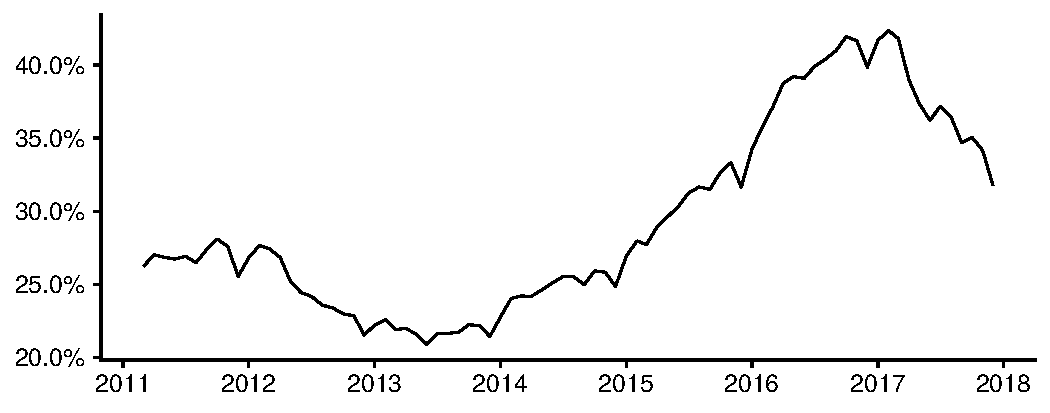
\includegraphics[width = \textwidth, scale=0.75]{Spread.pdf}
      \legend{Fonte: série 20786 do SGS. Elaboração própria}
      \label{spread}
\end{figure}

\bibliography{bibliografia}

\end{document}
